\documentclass{article}
\usepackage{amssymb}
\usepackage{mathtools}
\usepackage{verbatim}
\usepackage{physics}
\usepackage{tikz}
\usepackage{tikz-3dplot}

\usetikzlibrary{arrows}

\newcommand{\fig}[1]{Figure. #1}
\usepackage[utf8]{inputenc}
\newcommand{\vect}[1]{\boldsymbol{#1}}
\title{basic functions analytic hamiltonians}
\begin{document}
For a molecule with $N$ atoms, let us parametrise the nuclear coordinates with three centre of mass coordinates $\{X,Y,Z\}$ in the laboratory-frame, three Eulerian angles $\{\theta, \phi, \psi\}$ which specify the orientation of the body-fixed frame with respect to the space-fixed frame, and $3N-6$ internal coordinates $\{q_1, \ldots, q_{3N-6}\}$. With this parametrisation, the nuclear kinetic energy operator is  
\[
\hat{T}= \dfrac12 \sum_{a,b}\hat{\pi}_a G_{ab}\hat{\pi}_b + U
\]
where the $\hat{\pi}$s are the momentum operators and $a$ and $b$ sum over all coordinates in the order specified. In this expression, both the $G$ matrix and pseudo potential $U$ are functions only of the internal coordinates. We wish to express the components of $G$ and $U$ as a sum of 1D products of analytic functions of the coordinates, i.e. in the form
\[
\sum_{p} a_p f_{1i_1}(q_1)f_{2i_2}(q_2)\ldots f_{3N-6 i_{3N-6}}(q_{3N-6})
\]
where the $f$s are functions and $a_p$ is the coefficient with $p\in \{i_1, \ldots, i_{3N-6}\}$. In this expression, each $i_j$ denotes the $i$th function for the $j$th coordinate. The sum is over all such possibilities. 

This form generalises the current TROVE approach in which $f_{ij}(q_i) = (q_i)^j$ for all $i$ where the sum is over all $p$ and $p \in \{ i_1, \dots, i_{3N-6} | i_1 + \ldots + i_{3N-6} \leq P\}$ for some integer $n$, i.e. Taylor expanding the $G$ components and $U$ in each of the coordinates with a maximum overall power governed by $n$. Typically, the $q$s are linearised coordinates constructed from geometrically defined coordinates. 

This are two advantages to the newer approach. Evidently, the analytic Hamiltonian is exact and therefore should be expected to give more accurate results. Convergence typically is not achieved when Taylor expanding the Hamiltonian, even for `high' values of $n$, such as 6, which are only obtainable. Moreover, such large values of $n$ are only possible with small molecules due to the rate at which the number of terms increases with $n$. 

Related to this, the other benefit of the newer approach is the smaller number of terms in the Hamiltonian reduces the number of calculations that need to be performed during evaluation of matrix elements and recudes the disc space needed to store the Hamiltonian. This is particularly true if one of the coordinates, $\rho$, say, is treated as a non-rigid degree of freedom, so that $a_p(\rho)$ becomes a function of $\rho$ to be evaluated at a grid of points. A typical value of 1000 points inreases the number of terms in the Hamiltonian by the same factor. An analytic Hamiltonian does away with needing to express $a_p$ as a function of another coordinate, even a non-rigid one. 

When evaluating matrix elements $\matrixel{\psi_i}{G}{\psi_j}$ and $\matrixel{\psi_i}{U}{\psi_j}$, where $\ket{psi_i}$ are the basis functions written also a sum of 1D products of functions of the coordinates, the former method stores certain elemantary integrals, namely
\[
	\begin{split}
		&\matrixel{\nu_i}{(q_i)^j}{\nu_i'} \\
		&\matrixel{\nu_i}{(q_i)^j\hat{\pi}_i}{\nu_i'} \\
		&\matrixel{\nu_i}{\hat{\pi}_i (q_i)^j}{\nu_i'} = - \matrixel{\nu_i}{(q_i)^j \hat{\pi}_i}{\nu_i'}\\
		&\matrixel{\nu_i}{\hat{\pi}_i (q_i)^j\hat{\pi}_i}{\nu_i'} \\
	\end{split}
\]
where $\ket{\nu_i}$ is the $\nu$th excitation for the $i$th coordinate. This allows the matrix elements to be obtainable through only algebraic manipulations of the elementary integrals. Thus we see that this is crucial in the newer method for the terms to be separable so that all integrals reduce to a sum of products of 1D integrals. With the newer approach, however, the lower number of terms also greatly reduces the number of algebraic manipulations required. 

In this paper, we shall demonstrate, when one is restricted to valence coordinates, that there is a finite list of possible functions $f$ that is present in $G$ and $U$ and that this list is independent of the molecule, although it does depend on the body-fixed frame in a systematic way.   

To do so, we shall largely follow Sorensen's method for obtaining the Hamiltonian, which we will briefly outline. The $G$ matrix and pseudo potential $U$ are given by
\[
\begin{split}
G_{ab} &= \sum_{\alpha} \frac{1}{m_\alpha}\vect{s}_{a, \alpha}\cdot \vect{s}_{b, \alpha} \\
U &= \dfrac14 \sum_{ab \alpha i} \frac{1}{m_\alpha}(s_{a,\alpha i}[\hat{\pi}_a,[\hat{\pi}_b, s_{b,\alpha i}]] + \dfrac12 [\hat{\pi}_a, s_{a,\alpha i}][\hat{\pi}_b, s_{b,\alpha i}]) \\
\end{split}
\]
where $\alpha \in \{ 1, \ldots, N \}$ ranges over the atoms, $m_{\alpha}$ is the mass of the $\alpha$th atom, and $i \in \{ x,y,z\}$ ranges over the three components of $\vect{s}_{a,\alpha}$. The $s$-vectors are extracted from the $s$ matrix, the inverse of the $t$ matrix: the $a$th row of $s$, say, is given by $\vect{s}_{a}$. This is then further separated into groups of three (by atom) so that $\vect{s}_{a}$ is the $a$th row of $s$ and $\vect{s}_{a, \alpha}$ the $\alpha$th group of $\vect{s}_a$. A similar convention will be used for the $t$-vectors, with the difference that $\vect{t}_a$ is the $a$th \emph{column} of $t$. A note on notation: rotational, vibrational, and translation $s$ and $t$ vectors are labelled with $\{g, h\}$, $k$, and $F$, respectively. General components of these vectors are labelled with other letters, and atoms are labelled by $\{\alpha, \beta\}$.  

The $t$ matrix itself is constructed from three types of vectors,
\[
\begin{split}
    \vect{t}_{F,\alpha} &= \vect{e}_F  \text{(translations)} \\
    \vect{t}_{g, \alpha} &= \vect{e}_g \times \vect{r}_\alpha \text{(rotations)} \\
    \vect{t}_{k,\alpha} &= \pdv{\vect{r}_\alpha}{q_k} \text{(vibrations)} 
\end{split}
\]
where $\vect{e}_F$ is the unit vector in the $F$ direction and $\vect{r}_\alpha$ is the Cartesian coordinate of atom $\alpha$ in the centre of mass frame. One can immediately calculate the corresponding translational and vibrational $s$-vectors,
\[
\begin{split}
    \vect{s}_{F,\alpha} &= \frac{m_\alpha}{M}\vect{e}_F \text{(translations)} \\
    \vect{s}_{k, \alpha} &= \nabla_\alpha q_k \text{(vibrations).} \\
\end{split}
\]

To obtain the rotational $s$-vectors requires further work. One first defines three constraints defined from the orientation of the axes: 
\[
C^{(g)}(r_{1x}, r_{1y}, \ldots, r_{Nz}) = 0
\]
where $g \in \{x,y,z\}$, although the ordering of the conditions is irrelevant. One then creates a new set of vectors given by 
\[
\vect{c}_{g, \alpha} = \sum_{g'}\vect{e}_{g'}\pdv{C^{(g)}}{r_{\alpha g'}}
\]
with $g' \in \{x,y,z\}$.  Using these and the rotational $t$-vectors, one can construct the $J$ matrix:  
\[
J_{g g'} = \sum_{\alpha} \vect{c}_{g, \alpha}\cdot  \vect{t}_{g', \alpha}.
\]
The rotational $s$-vectors can then finally be determined and are given by 
\[
\vect{s}_{g, \alpha} = \sum_{g'} J^{-1}_{g g'} \vect{c}_{g', \alpha}. 
\]
One further point that to note is that the $\vect{c}$ vectors must satisfy the requirement that
\[
\sum_{\alpha} \vect{c}_{g, \alpha} = 0.
\]
If they do not, they can be readily adjusted to $\vect{c}'$ via
\[
\vect{c}'_{g, \alpha} = \vect{c}_{g, \alpha} -\frac{m_\alpha}{M} \sum_{\alpha'} \vect{c}_{g, \alpha'} 
\]
where $M$ is the sum of the nuclear masses. This does not affect the other necessary conditions. 

It is apparent that one only needs to show that the $s$ matrix has the desired form as constructructing the $G$ matrix and $U$ from it does not break this form. To demonstrate our result, we shall first show how the $s$-vectors transform when the axes is translated and rotated. We will then calculate the $s$-vectors under the simplest conditions and use the transformation properties to re-express them when in the desired frame. 

First, we note that the translational vectors of $s$ and $t$ are invariant under rotation and translation. The vectors $\vect{r}_\alpha$ transform to $M\vect{r}_\alpha$ under rotation, where $M$ is the rotation matrix. Here we ignore translation since $\vect{r}_\alpha$ are assumed to be calculated with the origin at the centre of mass. Then, the vibrational $t$-vectors $\vect{t}_{k, \alpha}$ transform to 
\[
\vect{t}_{k , \alpha} = \pdv{\vect{r}_\alpha}{q_k} \to \vect{t}'_{k, \alpha} = \pdv{(M\vect{r}_\alpha)}{q_k} = M \vect{t}_{k, \alpha} + \pdv{M}{q_k}\vect{r}_\alpha.
\]

Next, we consider the vibrational $s$-vectors $\vect{s}_{k, \alpha}$. All internal coordinates $q_k$ are invariant under translation and rotation, i.e.
\[
q_k(M\vect{r}_1 + \vect{d}, M\vect{r}_2 + \vect{d}, \ldots, M\vect{r}_N + \vect{d}) = q_k(\vect{r}_1, \vect{r}_2, \ldots, \vect{r}_N)
\]
where $\vect{d}$ is a displacement vector. Calling $T(\vect{r}) = M\vect{r} + \vect{d}$, and $\partial_{\alpha i}$ being the derivative of the argument of $q_k$ corresponding to component $i$ of atom $\alpha$, we want to determine $\partial_{\alpha i}(q_k)(T(\vect{r}_1), \ldots, T(\vect{r}_N))$ in terms of $\partial_{\alpha i}(q_k)(\vect{r}_1, \ldots, \vect{r}_N)$, that is, the $\alpha i$ derivative evaluated at the transformed coordinates in terms of the derivative evaluated at the un-transformed coordinates. Let us define the function $\tilde{T}$ as
\[
\Tilde{T}(\vect{r}_1, \ldots \vect{r}_N) = (T\vect{r}_1, \ldots, T\vect{r}_N).
\]
Then, the translational and rotational invariance can be expressed as 
\[
q_k \circ \tilde{T}(\vect{r}_1, \ldots, \vect{r}_N) = q_k(\vect{r}_1, \ldots, \vect{r}_N).
\]
Differentiating both sides, and using the chain rule, we obtain
\[
\partial_{\alpha i}(q_k)(\vect{r}_1, \ldots, \vect{r}_N) =\partial_{\alpha i} (q_k \circ \tilde{T})(\vect{r}_1, \ldots, \vect{r}_N)) 
\]
\[
= \sum_{\beta} \partial_{\alpha i}(T)^{\beta j}(\vect{r}_1, \ldots, \vect{r}_N)\cdot 
\partial_{\beta j}(q_k)(T(\vect{r}_1, \ldots, \vect{r}_N)
\]
where $\beta \in \{1, \ldots, N\}$ is over the atoms and $j \in \{x, y, z\}$ is over the coordinates, the latter using Einstein's summation convention. Here $\partial_{\alpha i}(\tilde{T})^{\beta j}$ is the $\beta j$ component of the derivative of $\tilde{T}$, which is nonzero only when $\beta =\alpha$ and is given by $M_{ji}$. We thus have 
\[
\partial_{\alpha i}(q_k)(\vect{r}_1, \ldots, \vect{r}_N) =  M_{ji}\partial_{\alpha j}(q_k)(\tilde{T}(\vect{r}_1, \ldots, \vect{r}_N)
\]
which can be inverted to give
\[
\partial_{\alpha m}(q_k)(\tilde{T}(\vect{r}_1, \ldots, \vect{r}_N)) = M_{mi}\partial_{\alpha i}(q_k)(\vect{r}_1, \ldots, \vect{r}_N).
\]
This is the required result. Thus
\[
\vect{s}_{k, \alpha} = \nabla_{\alpha}q_k \to \vect{s}'_{k, \alpha} = M\vect{s}_{k, \alpha}
\]
which means they transform as the Cartesian coordinates. 

We must also check the rotational $t$ and $s$ vectors behave properly as inverses:
\[
\begin{split}
\delta_{kk'} &= \sum_{\alpha} \vect{s}'_{k, \alpha}\cdot \vect{t}'_{k', \alpha} = \sum_{\alpha}  M\vect{s}_{k, \alpha}\cdot M\vect{t}_{k', \alpha} +  M\vect{s}_{k, \alpha}\cdot \pdv{M}{q_{k'}}\vect{r}_\alpha \\ &= \delta_{kk'} + \sum_{\alpha}  M\vect{s}_{k, \alpha}\cdot \pdv{M}{q_{k'}}\vect{r}_\alpha \\
\end{split}
\]
implying
\[
\sum_{\alpha}  M\vect{s}_{k, \alpha}\cdot \pdv{M}{q_k'}\vect{r}_\alpha  =\sum_{\alpha} M_{ij} s_{k, \alpha j}\pdv{M_{im}}{q_{k'}}r_{ \alpha m}= 0.
\]
where the middle expression was written using Einstein's summation convention. We also note that the invariance of the vibrational $G$ elements is satisfied, as expected. 

To determine the transformation of the rotational $s$-vectors, we first calculate the transformation of the rotational $t$-vectors, which are 
\[
t_{g, \alpha i} = \varepsilon_{igj}r_{\alpha j} \to t'_{g, \alpha i} = \varepsilon_{igj} M_{jm}r_{\alpha m}.
\]
This can be expressed in terms of the original $t$ vectors:
\[
\begin{split}
t'_{g,\alpha i} &= M_{gh} t_{h, \alpha j} M_{ij} = M_{gh} M_{ij} \varepsilon_{jhm} r_{\alpha m} \\&= M_{gh} M_{ij} M_{pn} \varepsilon_{ihn} M_{pm} r_{\alpha m} = \det(M) \varepsilon_{igp} M_{pm} r_{\alpha m} = \varepsilon_{igp} M_{pm} r_{\alpha m}.
\end{split}
\]
Viewing $\vect{t}_{g, \alpha}$ as the matrix $t_{\text{r},\alpha}$, where $g$ signifies the coloumns, this can be expressed as 
\[
t'_{\text{r}, \alpha} = Mt_{\text{r}, \alpha}M^{T}.
\]
For the transformation of the rotational $s$ vectors, we assert that they become
\[
s_{g, \alpha i} \to s'_{g, \alpha i} = M_{gh} M_{ij} s_{h, \alpha j} - 
\sum_{\beta} \pdv{M_{mn}}{q_{k}}s_{k, \alpha j} s_{h, \beta p} M_{mp} r_{\beta n} M_{ij} M_{gh} 
\]
where $k \in \{1, \ldots, 3N-6\}$ ranges over the vibrational coordinates and $\beta \in \{1, \ldots, N\}$ ranges over the atoms. Viewing $\vect{s}_{g, \alpha}$ as the matrix $s_{\text{r},\alpha}$, where $g$ is the column, this can also be written as 
\[
	s'_{\text{r}, \alpha} = Ms_{ \text{r}, \alpha}M^T - \sum_{\beta k} (M\vect{s}_{k, \alpha})\cdot\left(M s_{ \text{r}, \beta} M^T \pdv{M}{q_{k}}\vect{r}_\beta \right)^T.
\]
To demonstrate that this is the correct transformation, we will show that this is the inverse of the transformed $t$ matrix. First, with the translational $t$-vectors, we have
\[ \begin{split}
\sum_{\alpha} t'_{F, \alpha i} s'_{g, \alpha i} &= \sum_\alpha \delta_{Fi} M_{gh} M_{ij} s_{h, \alpha j} - \delta_{Fi} \sum_{\beta} \pdv{M_{mn}}{q_{k'}}s_{k', \alpha j} s_{h, \beta p} M_{mp} r_{\beta n} M_{ij} M_{gh} \\
&= M_{gh}M_{Fj} \underbrace{\sum_\alpha s_{h, \alpha j}}_{=0} - M_{mp}M_{Fj}M_{gh}\pdv{M_{mn}}{q_{k'}}\sum_\beta s_{h, \beta p} r_{\beta n} \underbrace{\sum_\alpha s_{k', \alpha j}}_{=0}
\end{split}
\]
where both terms are zero due to the condition on the rotational and vibrational $s$-vectors. For the rotational $t$-vectors, have have
\[
\begin{split}
 \sum_{\alpha} t'_{g', \alpha i} s'_{g, \alpha i} &= M_{g'h'} M_{im} M_{gh} M_{ij} s_{h, \alpha j}t_{h', \alpha m}  \\ &
-\sum_\alpha  M_{g'h'} M_{im} t_{h', \alpha m}\sum_{\beta} \pdv{M_{pn}}{q_{k}}s_{k, \alpha j} s_{h, \beta l} M_{pl} r_{\beta n} M_{ij} M_{gh}. \\
\end{split}
\]
The first term equals 
\[
\sum_\alpha M_{g'h'} M_{im} M_{gh} M_{ij} s_{h, \alpha j}t_{h', \alpha m}  = M_{g'h'}M_{gh} \sum_\alpha \delta_{mj} s_{h, \alpha j}t_{h', \alpha m} = M_{g'h'}M_{gh}  \delta_{h'h} = \delta_{g'g},
\]
while the second is zero as
\[
\begin{split}
&\sum_\beta M_{g'h'} M_{gh} \pdv{M_{pn}}{q_{k}} s_{h, \beta l} M_{pl} r_{\beta n} \sum_\alpha M_{ij} M_{im} s_{k, \alpha j} t_{h', \alpha m} \\ &= \sum_\beta M_{g'h'} M_{gh} \pdv{M_{pn}}{q_{k}} s_{h, \beta l} M_{pl} r_{\beta n} \underbrace{\sum_\alpha  s_{k, \alpha j} t_{h', \alpha j}}_{=0}.
\end{split}
\]
Finally, for the vibrational $t$ vectors, we have 
\[
\begin{split}
\sum_\alpha  t'_{k, \alpha i}s'_{g, \alpha i} = \sum_\alpha &\left(M_{ij}t_{k, \alpha j} + \pdv{M_{ij}}{q_{k}}r_{\alpha j} \right) \times \\&\left( M_{gh} M_{il} s_{h, \alpha l} - 
\sum_{\beta} \pdv{M_{mn}}{q_{k'}}s_{k', \alpha l} s_{h, \beta p} M_{mp} r_{\beta n} M_{il}M_{gh}\right)\\
\end{split}.
\]
Combining the first term from each, we obtain
\[
\sum_\alpha M_{ij}M_{gh} M_{il}t_{k,\alpha j}s_{h, \alpha l} =M_{gh}\underbrace{\sum_\alpha t_{k, \alpha j}
s_{h, \alpha j}}_{=0}.
\]
 Combining the second term from each, we get
\[
-\sum_\beta \pdv{M_{mn}}{q_{k'}}s_{h, \beta p} r_{\beta n} M_{mp} M_{gh} \underbrace{\sum_\alpha M_{il} s_{k', \alpha l} \pdv{M_{ij}}{q_k} r_{\alpha j}}_{=0}
\]
where the braced expression is zero due to identity X. Combining the second term in the first bracket with the first term in the second bracket, we have 
\[
\sum_\alpha \pdv{M_{ij}}{q_k}r_{a j} M_{gh} M_{il} s_{h, \alpha l}
\]
which in general is non-zero. However, combining the remaining two together, we obtain
\[
\begin{split}
&-\sum_{\beta} \pdv{M_{mn}}{q_{k'}}s_{h, \beta p} M_{mp}r_{\beta n} M_{gh}\sum_\alpha M_{ij}M_{il} t_{k,\alpha j} s_{k', \alpha l} \\&= -\sum_\beta \pdv{M_{mn}}{q_{k'}}M_{mp}r_{\beta n} s_{h, \beta o} M_{gh} \delta_{kk'} = -\sum_\beta \pdv{M_{mn}}{q_{k}}r_{\beta n} M_{gh}M_{mp} s_{h, \beta p}  \\
\end{split}
\]
which cancels with the other non-zero term.  

\begin{comment}
Using these expressions, we determine how the other $G$ matrix components transform. The rotational components become
\[
\begin{split}
G_{gg'} \to G_{gg'}' = \sum_{\alpha}\frac{1}{m_\alpha}&\left( M_{gh}M_{ij}s_{h, \alpha j} -\sum_{\beta} \pdv{M_{mn}}{q_{k}}s_{k, \alpha j} s_{h, \beta p} M_{mp} r_{\beta n} M_{ij} M_{gh} \right)\times \\&  
\left( M_{g'h'} M_{il} s_{h', \alpha l}- \sum_{\gamma} \pdv{M_{uv}}{q_{k'}}s_{k', \alpha l} s_{h', \gamma o} M_{uo} r_{\gamma v} M_{il} M_{g'h'} \right)
\end{split}
\]
Combining the first two terms gives
\[
M_{gh}M_{g'h'} \sum_\alpha \frac{1}{m_\alpha}s_{h, \alpha j} s_{h', \alpha j} = M_{gh} M_{g'h'} G_{hh'} = MG_{\text{rot}}M^T
\]
where in the last expression we wrote the rotational part of $G$ as the $3\times 3$ matrix $G_\text{rot}$. When we combine the last two terms of each, we obtain
\[
\begin{split}
&\sum_{\beta, \gamma} \pdv{M_{mn}}{q_k}\pdv{M_{uv}}{q_{k'}} M_{gh}s_{h, \beta p} M_{g'h'}s_{h', \gamma o} M_{mp} M_{uo} r_{\beta n} r_{\gamma v} \sum_\alpha \frac{1}{m_\alpha} s_{k', \alpha l} s_{k, \alpha l} =\\
& G_{k'k} \left( \sum_{\beta} \pdv{M_{mn}}{q_k} M_{mp}M_{gh} s_{h, \beta p} r_{\beta n}\right)\left( \sum_{\gamma} \pdv{M_{uv}}{q_{k'}} M_{qw}M_{g'h'} s_{h', \gamma o} r_{\gamma v}\right) \\
 \end{split}
 \]
 which can be written as 
 \[
 \sum_{k k'} G_{k'k} \sum_{\alpha \beta} \left(  M s_{\text{r}, \alpha} M^T \pdv{M}{q_k}\vect{r}_\alpha \right) \cdot  \left(  M s_{\text{r}, \beta} M^T \pdv{M}{q_k}\vect{r}_\beta \right)^T
 \]
The other two terms are zero:
\[
-\sum_{\alpha}\frac{1}{m_\alpha}M_{gh} \pdv{M_{uv}}{q_{k'}}s_{h', \gamma o} M_{uo} r_{\gamma v} M_{g'h'} \underbrace{\sum_\gamma s_{k', \alpha l} s_{h, \alpha l}}_{=0}.
\]

Finally, the Coriolis components become
\[ 
\begin{split}
G_{kg} \to G'_{kg} &= \sum_{\alpha} \frac{1}{m_\alpha}M_{il}s_{k, \alpha l} \left( M_{gh}M_{ij}s_{h, \alpha j} -\sum_{\beta} \pdv{M_{mn}}{q_{k'}}s_{k', \alpha j} s_{h, \beta p} M_{mp} r_{\beta n} M_{ij} M_{gh} \right) \\
&M_{gh} G_{kh} -  M_{g h} G_{kk'} \sum_\beta \pdv{M_{mn}}{q_{k'}} s_{h, \beta p} M_{mp} r_{\beta n}.
\end{split} 
\]
Viewing $G_{kh}$ as a vector $\vect{G}_k$, this can be written as
\[
M\vect{G}_k -\sum_{k'}G_{kk'} \sum_\beta M s_{\text{r}, \beta}M^T \pdv{M}{q_k'}\vect{r}_\beta.
\]
From these expressions it is clear that in practical calculations, one would work out 
\[
 M s_{\text{r}, \alpha}M^T \pdv{M}{q_k}\vect{r}_\alpha \text{ and}
\]
\[
M\vect{s}_{k, \alpha}
\]
for all $\alpha \in \{1, \ldots, N\}$ and $k \in \{1, \ldots, 3N-6\}$ and then sum them in the appropriate way to calculate the change in the $G$ matrix. 
\end{comment}

Now that we have derived the transformation properties of the $s$-vectors, we may determine the $s$-vectors in the frame where they are simplest and use the properties to express them in the desired frame. Initially, we assume that our desired body-fixed frame is oriented as in \fig{\ref{fig:initial_frame}}, where $a$, $b$, and $c$ are the first atoms in the Z-matrix.   
\begin{figure}[htbp!]
    \centering
    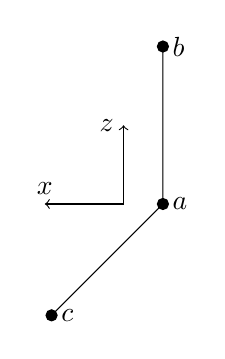
\begin{tikzpicture}
		\filldraw[-] (-1.4141,-1.4141,0) circle(2pt) node[right] {$c$} -- (0,0,0) circle(2pt) node[right] {$a$} --(0,2,0) circle(2pt) node[right] {$b$};
		\draw[<->] (-1.5,0,0) node[above] {$x$} -- (-0.5,0,0) -- (-0.5,1,0) node[left] {$z$};
    \end{tikzpicture}
    \caption{The initial frame that will be used in determining the $s$-vectors.}
    \label{fig:initial_frame}
\end{figure}

\begin{subsection}{Internal Coordinates}
As mentioned, we will demonstrate our result for valence coordinates. 
\begin{subsubsection}{Bond Length}
We assume we have two atoms, $a$ and $b$, with $a$ at the origin and $b$ lying along the z axis, i.e. $\vect{r}_a = (0,0,0)$ and $\vect{r}_b = (0,0,r_b)$ where $r_b = |\vect{r}_{ba}| = |\vect{r}_b - \vect{r}_a|.$ The equation for the bond length is given by 
\[
	R = \sqrt{(r_{ax} - r_{by})^2 + (r_{ay} - r_{by})^2 + (r_{az} - r_{bz})^2}.
\]
Calling this function $R$, the required derivatives are given by, once we substitute the Cartesian coordinates expressed in terms of internal coordinates, 
\[
\begin{split}
	\pdv{R}{r_{az}} &= -1 \\
	\pdv{R}{r_{bz}} &= 1 \\
\end{split}
\]
with the rest being zero, so in this case there is no function of the internal coordinates in the vibrational part of $s$. 
	
For the bond between atoms $a$ and $c$, we merely need to find the rotation matrix that rotates the coordinates when the $z$ axis is along $a$ to $c$ and the $x$ axis is still along plane of atoms $a$, $b$, and $c$, i.e. along the planar angle generated from these atoms. This matrix is given by
\begin{equation}
\label{angle-matrix}
\begin{pmatrix}
\cos\phi_{a}& 0 & -\sin\phi_{a} \\
0 & 1 & 0 \\
	\sin\phi_{a}& 0 & \phantom{-}\cos\phi_{a}
\end{pmatrix}
\end{equation}
	where $\phi_a$ is the planar angle between $c$, $a$, and $b$. Multiplying this by our previously derived vibrational $s$-vectors (with the appropriate atom replacements), we see that it introduces $\sin \phi_b$ and $\cos\phi_a $ to the vibrational $s$-vectors, and so these are added to our list of functions. When adding the fourth atom, where the angle and dihedral angle in the Z-matrix is $\phi$ and $\theta$, respectively, first one rotates about the current $z$ axis so that the $x$ axis is in the other dihedral angle plane, which has the transformation matrix given by
	\begin{equation}
	\label{eq:dihedral_mat}
		\begin{pmatrix}
\cos \theta & \sin \theta & 0 \\
-\sin \theta & \cos \theta & 0 \\
0 & 0 & 1
\end{pmatrix}
	\end{equation} 
and then one rotates about the $y$ axis so that the $z$ axis is parallel to the bond, and again the rotation matrix is
\[
\begin{pmatrix}

\pm\cos \phi & 0 & -\sin \phi \\
0 & 1 & 0 \\
\sin \phi & 0 &\pm\cos \phi   \\
\end{pmatrix}.
\]
	where the $\pm$ on the consines depends on the geometry of the molecule. That is, it depends on whether the rotation angle is $\phi$ or $\pi - \phi$. We apply the inverse transformation of this product. For an arbitrary atom, we make a string of products of this type $M_1\ldots M_n$ (starting from the last atom and working backwards) on the initially calculated vibrational $s$-vector until we reach the desired frame. Since each $M$ contains differing internal coordinates, to determine the functions of the coordinates, one must only take note of the functions in the matrix. Thus, it is clear that, for the bond length, the functions obtained are sines and cosines of the angles and the dihedral angles.    
\end{subsubsection}
\begin{subsubsection}{Planar Angles}
The formula for the angle between atoms $a$, $b$, and $c$ is 
\[
	\arccos \left ( \frac{\vect{r}_{ba} \cdot \vect{r}_{ca} }{r_b r_c} \right ) = 
\]
	where $r_c = |\vect{r}_{ca}|$.  $a_x$. We shall assume the same coordinate values for these atoms as for the bond length case. If $\varphi$ is the angle equation, the substituted derivatives are\[
\begin{split}
	\pdv{\varphi}{r_{ax}} &= \frac{1}{r_{b}} - \frac{\cos \phi_a}{r_c} \\
	\pdv{\varphi}{r_{az}} &=  -\pdv{\varphi}{c_z} =  \frac{\sin \phi_a}{r_c} \\ 
	\pdv{\varphi}{r_{bx}} &= -\frac{1}{r_{b}} \\
	\pdv{\varphi}{r_{cx}} &= \frac{\cos\phi_{a}}{r_{c}} \\ 
\end{split}
\]
with the rest being zero. It is clear that $1/r$ type functions have to be added to the list of possibilities, where $r$ is a bond length. 
\end{subsubsection}
	\begin{subsubsection}{Dihedral Angles}
		For dihedral angles, another atom, $d$, has to be added, as shown in \fig{\ref{fig:fourthatom}}. The atom could also be connected to $a$ rather than $d$, but this does not change the conclusion of the results.  
\begin{figure}[htbp!]
\centering
	\tdplotsetmaincoords{70}{120}{0}
\begin{tikzpicture}[tdplot_main_coords]
	\filldraw[-] (1.4141,0,-1.4141) circle(2pt) node[right] {$c$} -- (0,0,0) circle(2pt) node[right] {$a$} --(0,0,2) circle(2pt) node[right] {$b$} --  (-1.1547, 1.1547, 1.1547 +2) circle(2pt) node[right] {$d$};
		\draw[<->] (1.5,0,0) node[above] {$x$} -- (0.5,0,0) -- (0.5,0,1) node[left] {$z$}; 
		\draw[->] (0.5,0,0) -- (0.5,1,0) node[above] {$y$};

\end{tikzpicture}
	\caption{The initial frame with the fourth atom added.}
	\label{fig:fourthatom}
\end{figure}	
		The coordinates are 
\[
\begin{split}
	\vect{a} &= (r_{c} \sin\phi_{a}, 0, r_{c} \cos \phi_{a})\\
    \vect{b} &= (0,0,0) \\
    \vect{c} &= (0,0,r_{c}) \\
	\vect{d} &= (r_{d} \cos\theta \sin\phi_b, r_{d} \sin\theta \sin\phi_{b},r_{b} - r_{d}\cos\phi_c) 
\end{split}
\]
		where, $r_d = |\vect{r}_{dc}|$, $\phi_b$ planar angle between  $a$, $b$, $d$, and $\theta$ is the dihedral angle. The equation for the dihedral angle is given by  
\[
\begin{split}
	\arctan&[(\vect{r}_{ba}\times \vect{r}_{ca})\cdot (\vect{r}_{ba} \times \vect{r}_{db}) r_b,  (\vect{r}_{ba} \times  (\vect{r}_{ba} \times \vect{r}_{ca}))\cdot (\vect{r}_{ba} \times \vect{r}_{db})] =\\
\arctan&[   (\vect{r}_{ba}\cdot\vect{r}_{ba})(\vect{r}_{db}\cdot\vect{r}_{ca}) - (\vect{r}_{ba}\cdot\vect{r}_{ca})(\vect{r}_{ba}\cdot\vect{r}_{db}),\\
	&r_b(\vect{r}_{ba}\cdot(\vect{r}_{ca} \times \vect{r}_{db})) ] \\
\end{split}
\]
and the substituted derivatives are given by
\[
\begin{split}
	\pdv{\theta}{r_{ax}} &= - \frac{\sin\theta}{r_{b}\tan\alpha_{c}}   \\
	\pdv{\theta}{r_{ay}} &= -\frac{1}{r_b \tan \alpha_a} - \frac{\cos \theta}{r_b\tan \alpha_c} + \frac{1}{r_c \sin \alpha_a} \\
	\pdv{\theta}{a_{bx}} &= - \frac{\sin \theta}{r_b \tan \alpha_c} + \frac{\sin \theta}{r_d \sin \alpha_c} \\
	\pdv{\theta}{r_{by}} &= \frac{1}{r_b \tan \alpha_a} + \frac{\cos \theta}{r_b\tan \alpha_c} - \frac{\cos \theta}{r_d \sin \alpha_c} \\
	\pdv{\theta}{r_{cy}} &= -\frac{1}{r_c \sin \alpha_a} \\
	\pdv{\theta}{r_{dx}} &= -\frac{\sin \theta}{r_d \sin \alpha_c} \\
	\pdv{\theta}{r_{dy}} &= \frac{\cos \theta}{r_d \sin \alpha_c} \\
\end{split}
\]
with the rest being zero. From these it is clear that the additional functions the dihedral angle generates are cosec and $\cot$ of the angles (but not dihedral angles).
In the general case, to arrive at the coordinate system this was calculated in, we have to transform the coordinates via a matrix containing $\sin \phi_a$ and $\cos \phi_a$, for the analogous $\phi_a$ in the general case, which could in principle generate new functions. However, all multiplications can be expressed in preexisting coordinates, the most complex of which is $\cos \cot = \csc - \sin$.
	\end{subsubsection}
	\end{subsection}
\begin{subsection}{Rotational $s$-vectors}

	Following Sorensen's method, we must define three conditions on the frame that are always zero. Using our initial frame, as shown in \fig{\ref{fig:fourthatom}}, the conditions are 
	\[
		\begin{split}
			C^{(x)} &= r_{bx} - r_{ax} = 0 \\
			C^{(y)} &= r_{by} - r_{ay} = 0 \\
			C^{(z)} &= r_{cy} - r_{ay} = 0 \\
		\end{split}
	\]
	where the first two conditions signify that the $z$ axis lies along $a$ to $b$ and the third that $x$ lies along the plane of $b$, $a$, and $c$. Using the method outlined, the rotational $s$-vectors are, as matrices, given by
	\[
	\begin{split}
		s_{\text{r}, a} &= \begin{pmatrix}
		0 & 1/r_b & 0 \\
			-1/r_b &0 & 0 \\
			0 & \cot \phi_a/ r_b - \csc \phi_a r_c & 0 \\
	\end{pmatrix} \\
		s_{\text{r}, b} &= \begin{pmatrix}
		0 & -1/r_b & 0 \\
		1/r_b & 0 & 0 \\
		0 & -\cot \phi_a /r_b & 0 \\
	\end{pmatrix} \\
		s_{\text{r}, c} &= \begin{pmatrix} 
			0 & 0 & 0 \\
			& 0 & 0 0 \\
			0 & - \cot \phi_a/r_c & 0 \\
		\end{pmatrix} \\
		s_{\text{r}, d} &= \begin{pmatrix}
			0 & 0 & 0 \\
			0 & 0 & 0 \\
			0 & 0 & 0 \\
		\end{pmatrix} \\
	\end{split}
	\]
and thus we see that the rotational $s$-vectors do not introduce new functions of the coordinates in this frame. For an arbitrary number of atoms, all other rotational $s_{\text{r}, \alpha}$ matrices are zero as beyond $\alpha = 3$ the vectors $\vect{c}_{g, \alpha}$ are zero. 
\end{subsection}
\begin{subsection}{Complete set of functions of the coordinates}
	In summary, for the $s$-vectors, the functions for the bond lengths, planar angles, and dihedral angles $r$, $\phi$, and $\theta$ in the initial frame are:
	\begin{itemize}
		\item Bond Lengths: $1/r$ 
		\item Planar Angles: $\cos \phi$, $\sin \phi$, $\cot \phi$, $\csc \phi$ 
		\item Dihedral Angles: $\sin \theta$, $\cos \theta$.
	\end{itemize}
In constructing the $G$ matrix and pseudo potential $U$, we must combine expressions of these functions. The $G$ matrix is given by 
	\[
		G_{ab} = \sum_{\alpha} \frac{1}{m_\alpha}\vect{s}_{a, \alpha}\cdot \vect{s}_{b, \alpha}
	\]
so we see we must multiply each function in a set with every function of the set. For the pseudo potential $U$, it can be shown to consist of 4 terms:
\[
	\begin{split}
		U_1 &= \frac{1}{8} \sum_{\alpha, g, g'} \frac{1}{m_\alpha} (\vect{e}_{g} \times \vect{s}_{g, \alpha})\cdot(\vect{e}_{g'} \times \vect{s}_{g', \alpha}) \\
		U_2 &= -\frac{1}{4} \sum_{\alpha, g, k}\frac{1}{m_\alpha} \left(\vect{e}_g \times \vect{s}_{k, \alpha}\right)\cdot \pdv{\vect{s}_{g, \alpha}}{q_k}  \\ 
		U_3 &= -\frac{1}{4} \sum_{\alpha, k, k'} \frac{1}{m_\alpha} \vect{s}_{k, \alpha}\cdot \pdv{\vect{s}_{k', \alpha}}{q_k}{q_{k'}} \\ 
		U_4 &= -\frac{1}{8} \sum_{\alpha, k, k'} \frac{1}{m_\alpha} \pdv{\vect{s}_{k, \alpha}}{q_k}\cdot \pdv{\vect{s}_{k', \alpha}}{q_{k'}} \\
	\end{split}
\]
where $U$ is the sum of these terms. From this, it is clear that we must also multiply first and second derivatives of each function in a set with every function of the set. However, in practice not all these combinations will actually be present in the Hamiltonian. 
\end{subsection}
\begin{subsection}{Arbitrary Frame}
	The previous analysis was for the frame being in the orientation shown in \fig{\ref{fig:fourthatom}}. The transformation properties make it apparent that when you rotate this frame, as long as the rotation matrix and its derivatives with respect to the internal coordinates have the same desired structure, that the $s$-vectors also remain in the desired form, albeit with potentially extra or alternative functions of the coordinates. It is not possible to make general remarks about the exact way a transformation alters which functions are present due to the complexity of the transformation, but a simplification of the transformation of the rotational $s$-vectors can be found when the rotation angle $\theta$ can be written as a function of the internal coordinates $\theta = f(q_1, \ldots, q_N)$. To maintain the separable nature of the Hamiltonian, $f$ must be of the form 
	\[
		\theta = f(q_1, \ldots, q_N) = f_1(q_1) + \ldots + f_N(q_N). 
	\]
for some $f_i$. If the rotation was about the $z$ axis, say, the rotation matrix is given by 
	\[
		\begin{pmatrix}
		\cos \theta & - \sin \theta & 0 \\
		\sin \theta & \cos \theta & 0 \\
		0 & 0 & 1 \\
		\end{pmatrix}
	\]
where a rotation of $\pi - \theta$ or $2\pi -\theta$ can easily be achieved by a corresponding
			adjustment of $f$ without spoiling the structure. Any arbitrary rotation can be obtained with a product of three rotation matrices. With this, the term $M^T \pdv*{M}{q_k}\vect{r}_\beta$ in the $s$-vector transformation becomes
\[
	\begin{split}
		M^T \pdv{M}{q_k}\vect{r}_\beta &= \pdv{f_k}{q_k}	\begin{pmatrix}
		\cos \theta &  \sin \theta & 0 \\
		-\sin \theta & \cos \theta & 0 \\
		0 & 0 & 1 \\
		\end{pmatrix} \begin{pmatrix}
		-\sin \theta & -\cos \theta & 0 \\
		\cos \theta & -\sin \theta & 0 \\
		0 & 0 & 0 \\ 
	\end{pmatrix}
			\begin{pmatrix}
			r_{\beta x} \\
			r_{\beta y} \\
			r_{\beta z} \\
			\end{pmatrix} \\
   &= \pdv{f_k}{q_k}   \begin{pmatrix}
                 0 & -1 & 0 \\
                 1 & 0 & 0 \\
                 0 & 0 & 0 \\
             \end{pmatrix}
             \begin{pmatrix}
                 r_{\beta x} \\
                 r_{\beta y} \\
                 r_{\beta z} \\
             \end{pmatrix}  = 
			\pdv{f_k}{q_k} \begin{pmatrix}
                 -r_{\beta y} \\
                 r_{\beta x} \\
                 0 \\ 
             \end{pmatrix} \\
		 &= \pdv{f_k}{q_k} (\vect{e}_z \times \vect{r}_\beta) = \pdv{f_k}{q_k} \vect{t}_{z, \beta}. \\
	\end{split}
\]
	Combining this with rest of the term, we have
	\[
		\sum_\beta M s_{\text{r}, \beta} \vect{t}_{z, \beta} = M \vect{e}_z = M_z
	\]
where $M_z$ is the third column of $M$. The final transformation is then 
	\[
		s'_{\text{r}, \alpha} = Ms_{\text{r}, \alpha} M^T - \sum_k \pdv{f_k}{q_k} (M\vect{s}_{k,\alpha})(M_z)^T.
	\]
We will now show an example of an alternative frame and how this changes the $s$-vectors. 
\end{subsection}
\begin{subsection}{Example frame}
	The first case is the $x$-axis bisecting the dihedral angle $\theta$. To transform to this frame requires matrix \ref{eq:dihedral_mat} but with $\theta$ replaced by $\theta/2$. For the atoms whose position does not require the dihedral, namely the first three, the vibrational $s$-vectors also did not contain $\theta$, so that applying the matrix merely introduces $\sin (\theta/2)$ and $\cos (\theta/2)$. For other atoms, the last matrix in the list $M_1 \ldots M_n$ is the inverse of \ref{eq:dihedral_mat}, and therefore, in multiplying these matrices, $\theta$ is replaced by $\theta/2$. Finally, when we apply the matrix on the $\theta$ dihedral $s$-vectors, we find again that the expressions are combined in such a way that the $s$-vectors only involve $\theta/2$ instead of $\theta$. 

	In practice, one would generate the $s$-vectors in this frame by straightforwardly substituting the derivatives with the correct Cartesian coordinates rather than applying the transformation. To that end, the conditions one would use are now given by
	\[
		\begin{split}
			C^{(x)} &= r_{by} - r_{ay}  = 0\\
			C^{(y)} &= r_{bx} - r_{ax}  = 0\\
			C^{(z)} &= (r_{cy} - r_{ay})(r_{dx} - r_{ax}) + (r_{cx} - r_{ax})(r_{dy} - r_{ay})
		\end{split}
	\]
	where the (different) third condition stems from the obseration that the tangent of the angle between from the $x$-axis to the bond $\vect{r}_c - \vect{r}_a$ projected onto the $xy$ plane (given by $(r_{cy} -r_{ay})/(r_{cx} - r_{ax})$ is negative the angle bteween the $x$-axis and the bond $\vect{r}_c - \vect{r}_a$ projected onto the $xy$ plane. Thus 
	\[
		\frac{r_{cy} - r_{ay}}{r_{cx} - r_{ax}} + \frac{r_{dy} - r_{ay}}{r_{dx} - r_{dx}} = 0
	\]
	and we multiply by the denominators to simplify the condition. With this, the rotational $s$-vectors we obtain depend on $\theta/2$ but not $\theta$, in other words the kinetic Hamiltonian no longer depends on $\theta$ at all. 

	A similar frame, that of the $z$ axis bisecting the first planar angle, can also be used. The results for the $s$-vectors are analogous to the bisecting $x$-axis example. 
\end{subsection}
\begin{comment}
The internal coordinates that will be considered are those arising during the construction of the Z-matrix, namely, bond lengths, angles, and dihedral angles. Without loss of generality, the origin of the Cartesian coordinate system may be the first atom in the Z-matrix.  To obtain all possible functions of the internal (vibrational) coordinates in the $s$ matrix, we shall differentiate the internal coordinates (written in terms of Cartesian coordinates) with respect to the Cartesian coordinates and evaluate these derivatives at the possible Cartesian coordinates expressed in terms of the internal coordinates. The coordinate axes in this case have the $z$ direction along the bond from the first to the second atom, and the $x$ axis lying in the plane of the bond from the third atom to the atom it's connected to (either the first or second atom). As the simplest example, if we call the Cartesian coordinates of the first and second atom $\vect{a}$ and $\vect{b}$, respectively, the equation of the bond length is given by
\[
\sqrt{(a_x - b_y)^2 + (a_y - b_y)^2 + (a_z - b_z)^2}.
\]
The derivative of this equation with respect to $b_z$ is
\[
\frac{(b_z - a_z)}{\sqrt{(a_x - b_x)^2 + (a_y - b_y)^2 + (a_z - b_z)}} = \frac{b_z - a_z}{|\vect{a} - \vect{b}|}
\]
with analogous derivatives for the other coordinates. With our assumptions, $\vect{a} = (0,0,0)$ and $\vect{b} = (0,0,r_{ab})$, where $r_{ab}$ is the bond length between atoms $a$ and $b$. Substituting this into the equation, we obtain
\[
\frac{r_{ab}}{r_{ab}} = 1, 
\]
so in this case there is no function of the internal coordinates in the vibrational part of $s$. Likewise, the derivative for $a_z$ is $-1$ and the others are all $0$. We shall now proceed with all the cases.

\section{Bond Length}
For the third atom $c$, there are two possibilities for its Cartesian coordinates $\vect{c}$. If $c$ is connected to $b$, its Cartesian coordinates are 
\[
\vect{c} = ( r_{bc} \sin(\alpha_{abc}),0, r_{ab} - r_{bc}\cos (\alpha_{abc})),
\] 
where $\alpha_{abc}$ is the angle between atoms $a$, $b$, and $c$. Differentiating the bond length with respect to $c_z$ and substituting, we obtain
\[
-\cos(\alpha_{abc})
\]
so that $\cos(\alpha_{abc})$ is the first function of an angular coordinate. We obtain $\sin(\alpha_{abc})$ by substituting the Cartesian coordinates of the derivative with respect to $c_y$. The derivatives with respect to $c_x$ are 0, and the derivatives with respect to the other atom merely swap the sign.

However, we could have also obtained this result by assuming the Coordinate system's origin is at $\vect{b}$ and has the $z$ axis in the $c$-$b$ bond direction. Then, using the transformation of the coordinates between these two systems 
\[\vect{c} = M \vect{c}' + \vect{d},\]
where $\vect{c}'$ is the list of components of the position in terms of the new system, $M$ is the rotation matrix between them, and $\vect{d}$ is their displacement, we see that the $\vect{s}$ component can also be expressed in the original system by
\begin{equation}
    \label{bond-s}
\frac{[M(\vect{c}' - \vect{b}')]_z}{|M(\vect{c}' - \vect{b}')|} = \frac{[M(\vect{c}' - \vect{b}')]_z}{|\vect{c}' - \vect{b}'|}
\end{equation}
where the numerator denotes the $z$ component. Since $\vect{d}$ drops out, it is irrelevant. In other words, the $\vect{s}$ component 
\[
\frac{\vect{c}' - \vect{b}'}{|\vect{c}' - \vect{b}'|} = \frac{\vect{c}' - \vect{b}'}{|\vect{c} - \vect{b}|}
\]
transforms the same way as the Cartesian coordinate components, i.e. through the rotation matrix $M$. 

The denominator in \ref{bond-s} is the equation for the bond length, so is simply $r_{bc}$. Here, $M$ is given by
\begin{equation}
\label{angle-matrix}
\begin{pmatrix}
-\cos(\alpha_{abc})& 0 & \phantom{-}\sin(\alpha_{abc}) \\
0 & 1 & 0 \\
 - \sin(\alpha_{abc})& 0 & -\cos(\alpha_{abc})
	\end{pmatrix}
\end{equation}
and $\vect{c}' = (0,0, r_{bc})$, $\vect{b}' = (0,0,0)$. The minus signs on the cosines arise because the rotation angle is $\pi - \alpha_{abc}$. Therefore, 
\[
[M(\vect{c}' - \vect{b}')]_z = -r_{bc}\cos(\alpha_{abc})
\]
and so we obtain the same result as previously. The other possibility is that $c$ was connected to the first atom, which would give it coordinates
\[
\vect{c} = (r_{ac} \sin(\alpha_{abc}), 0,  r_{ac}\cos (\alpha_{abc})),
\] 
and thus provide no new function of the vibrational coordinates. For extra atoms, it is more straightforward to find the transformation of the Coordinates that so that the $z$-axis is now along the bond of interest and the $k$-axis in the three atom plane of the dihedral angle which includes the added atom. Then the above procedure is followed. In the case of bond lengths, once the axes are in this position, the substituted derivatives can only be $1$, $-1$, or $0$. Afterwards, one makes a string of transformations $\vect{c} \to M \vect{c}' + d$ for all transformations of the Coordinates. Since each $M$ contains differing internal coordinates, to determine the functions of the coordinates, one must only take note of the functions in the matrix.

When adding the atoms after the third, where the angle and dihedral angle is $\alpha$ and $\theta$, respectively, first one rotates about the current $z$ axis so that the $x$ axis is in the other dihedral angle plane, which has the inverse transformation (which we are interestd in) matrix given by
\[
\begin{pmatrix}
\cos \theta & -\sin \theta & 0 \\
\sin \theta & \cos \theta & 0 \\
0 & 0 & 1
\end{pmatrix}
\] 
and then one rotates about the $y$ axis so that the $z$ axis is parallel to the bond, and again the rotation matrix is
\[
\begin{pmatrix}

-\cos \alpha & 0 & \sin \alpha \\
0 & 1 & 0 \\
-\sin \alpha & 0 &-\cos \alpha   \\
\end{pmatrix}.
\]
Thus, it is clear that, for the bond length, the functions obtained are sines and cosines of the angles and the dihedral angles.

\section{Angles}
The formula for the angle between atoms $a$, $b$, and $c$ is 
\[
\arccos \left ( \frac{(\vect{a} - \vect{b}) \cdot (\vect{c} - \vect{b})}{|\vect{a} - \vect{b}| |\vect{c} - \vect{b}|} \right ) = \arccos\left({\frac{x}{yz}}\right)
\]
with $x$ defined by the numerator and $y$ and $z$ being given by $|\vect{a} - \vect{c}|$ and $|\vect{c} - \vect{b}|$, respectively. As with the bond length, we want to show that the derivatives with respect to the Cartesian coordinates transforms through the same matrix as the Cartesian components. The function is symmetric in $\vect{a}$ and $\vect{c}$ so derivatives with respect to these have equivalent form, insofar as proving the transformation property. Differentiating with respect to $a_x$, we obtain
\[
\frac{-1}{\sqrt{1-x^2/(yz)^2}}\left[\frac{(c_x - b_x)}{yz} - \frac{(a_x - b_x)x}{y^3z} \right],
\]
and differentiating with respect to $b_x$, we obtain
\[
\frac{-1}{\sqrt{1-x^2/(yz)^2}}\left[\frac{(2b_x -a_x - c_x)}{yz} - \frac{(a_x - b_x)x}{y^3z} \right].
\]
These both have the required property. 

We shall assume the same coordinate values for these atoms as for the bond length case. If $\phi$ is the angle equation, the substituted derivatives are 
\[
\begin{split}
\pdv{\phi}{a_x} &= -\frac{1}{r_{ab}} \\
\pdv{\phi}{b_x} &= \frac{1}{r_{ab}} - \frac{\cos(\alpha_{abc})}{r_{bc}} \\
\pdv{\phi}{b_z} &= -\pdv{\phi}{c_z}= -\frac{\sin(\alpha_{abc})}{r_{bc}} \\
\pdv{\phi}{c_x} &= \frac{\cos(\alpha_{abc})}{r_{bc}} \\ 
\end{split}
\]
with the rest being zero. It is clear that $1/r$ type functions have to be added to the list of possibilities, where $r$ is a bond length. 

\section{Dihedral Angles}
For dihedral angles, it is most straightforward to have the axes' origin at the second atom, with the $z$ axis in the direction of the third atom and the $x$ axis lying in the first dihedral plane. Calling these atoms $a$, $b$, $c$, and $d$, and assuming $c$ is connected to $d$, the coordinates are 
\[
\begin{split}
    \vect{a} &= (r_{ab} \sin(\alpha_{abc}),0, r_{ab} \cos( \alpha_{abc})) \\
    \vect{b} &= (0,0,0) \\
    \vect{c} &= (0,0,r_{bc}) \\
    \vect{d} &= (r_{cd} \cos(\theta) \sin(\alpha_{bcd}), r_{cd} \sin(\theta) \sin(\alpha_{bcd}),r_{bc} - r_{cd}\cos(\alpha_{bcd})) 
\end{split}
\]
where $\theta$ is the dihedral angle. The equation for the dihedral angle is given by 
\[
\begin{split}
\arctan&[(\vect{r}_{cb}\times \vect{r}_{ab})\cdot (\vect{r}_{cb} \times \vect{r}_{dc}) \sqrt{\vect{r}_{cb} \cdot \vect{r}_{cb}},  (\vect{r}_{cb} \times  (\vect{r}_{cb} \times \vect{r}_{ab}))\cdot (\vect{r}_{cb} \times \vect{r}_{dc})] =\\
\arctan&[   (\vect{r}_{cb}\cdot\vect{r}_{cb})(\vect{r}_{ab}\cdot\vect{r}_{dc}) - (\vect{r}_{cb}\cdot\vect{r}_{ab})(\vect{r}_{cb}\cdot\vect{r}_{dc}) \\
&,\sqrt{\vect{r}_{cb}\cdot\vect{r}_{cb}} (\vect{r}_{cb}\cdot(\vect{r}_{ab} \times \vect{r}_{dc})) ] \\
\arctan&[u^2 w - x y, u z] 
\end{split}
\]
where $\vect{r}_{ab} = \vect{a} - \vect{b}$, and so on, and $u$, $w$, $x$, $y$, and $z$, are $(\sqrt{\vect{r}_{cb} \cdot \vect{r}_{cb}$), $(\vect{r}_{ab} \cdot \vect{r}_{dc})$, $(\vect{r}_{cb} \cdot \vect{r}_{ab})$, $(\vect{r}_{cb} \cdot \vect{r}_{dc})$, and $\vect{r}_{dc} \cdot (\vect{r}_{cb} \times \vect{r}_{ab})$, respectively. All these terms are invariant under rotation, the latter being the volume spanned by the three vectors. Also, note that $M\vect{a} \times M \vect{b} = M( \vect{a} \times \vect{b})$ for rotation matrices $M.$ The derivatives with respect to the Cartesian coordinates contain a prefactor 
\[
\frac{1}{(u^2 w -xy)^2 + (uz)^2} 
\]
which will not be explicitly written. Once again, the function is antisymmetric when $\vect{b}$ and $\vect{c}$ are swapped, and also when $\vect{a}$ and $\vect{d}$ are swapped. Thus, we only need to evaluate the derivatives with respect to $a$ and $b$. The derivative with respect to $a_x$ is given by 
\[
u(u^2w - xy) [\vect{r}_{dc} \times \vect{r}_{cb}]_x  -uz(u^2[\vect{r}_{dc}]_x -y[\vect{r}_{cb}]_x)
\]
and the derivative with respect to $b_x$ is given by 
\[
\begin{split}
&(u^2w-xy)\left( -\frac{z[\vect{r}_{cb}]_x}{u^3}  +u([\vect{r}_{dc} \times \vect{r}_{ab}]_x  + [\vect{r}_{cb} \times \vect{r}_{dc}]_x) \right) \\
&+ uz(w([\vect{r}_{cb}]_x +u^2 [\vect{r}_{dc}]_x - y([\vect{r}_{cb}]_x +[\vect{r}_{ab}]_x) -x[\vect{r}_{dc}]_x  )
\end{split}
\]
with corresponding derivatives for the $y$ and $z$ directions. Thus, the required property is satisfied. Calling the dihedral angle $\varphi$, the substituted derivatives are given by
\[
\begin{split}
\pdv{\varphi}{a_y} &= - \frac{1}{r_{cb}\sin(\alpha_{abc})}  \\
\pdv{\varphi}{b_x} &= \frac{\sin(\theta)}{r_{dc}\sin(\alpha_{bcd})} - \frac{\sin(\theta)}{r_{ab}\tan(\alpha_{abc})} \\
\pdv{\varphi}{b_y} &= \frac{\cos(\theta)}{r_{ab}\tan(\alpha_{bcd})} - \frac{\cos(\theta)}{r_{dc}\sin(\alpha_{bcd})} + \frac{1}{r_{cb}\sin(\alpha_{abc})} - \frac{1}{r_{ab}\tan(\alpha_{abc})} \\
\pdv{\varphi}{c_x} &=  \frac{\sin(\theta)}{r_{ab}\tan(\alpha_{bcd})} \\ 
\pdv{\varphi}{c_y} &= \frac{1}{r_{ab}\tan(\alpha_{abc})} - \frac{\cos(\theta)}{r_{ab}\tan(\alpha_{bcd})} \\
\pdv{\varphi}{d_x} &= \frac{\sin(\theta)}{r_{dc}\sin(\alpha_{bcd})} \\
\pdv{\varphi}{d_y} &= \frac{\cos(\theta)}{r_{dc}\sin(\alpha_{bcd})} \\
\end{split}
\]
with the rest being zero. From these it is clear that the additional functions the dihedral angle generates are cosec and $\cot$ of the angles (but not dihedral angles).
To arrive at the coordinate system this was calculated in, we have to transform the coordinates via a matrix containing $\sin \alpha_{abc}$ and $\cos \alpha_{abc}$, which could in principle generate new functions. However, all multiplications can be expressed in preexisting coordinates, the most complex of which is $\cos \cot = \csc - \sin$.

\section{Modification of the Functions due to the Axes' Orientation}

The functions generated thus far assume that the $z$ lies along a bond and the $x$ axis lies in the plane formed by the first three atoms, where atoms are labelled in alphabetical order, as previously. If one wants to orient the axes differently, a slight modification occurs to the functions of the coordinates that are present. We shall consider the alternative of $x$ axis bisecting the dihedral angle and with the $z$ axis bisecting the first angle, resulting in three possibilities, one being the current case. Since one is free to choose in which order to add the atoms when making the Z matrix, we assume that the initial $z$ axis is the `$z$' axis of the dihedral angle and also that the initial $x$ axis lies in the plane of the first angle. We also assume the $c$ is connected to $a$. To obtain the final combination of functions, one prepends the transformation matrix $M$, which transforms the initial orientation to the final orientation, to the string $M_1M_2M_3\ldots $ of matrix transformations. 

For the case of $z$ bisecting the first angle, the transformation is
\[
M = 
\label{angle-bisect}
\begin{pmatrix}
\cos(\alpha_{abc}/2) & 0 & \sin(\alpha_{abc}/2) \\
0 & 1 & 0 \\
-\sin(\alpha_{abc}/2) & 0 & \cos(\alpha_{abc}/2) \\
\end{pmatrix}.
\]
For any atom whose position involves $\alpha_{abc}$, $M_1$ is given by
\[
\label{angle-matrix-alt}
M_1 = 
\begin{pmatrix}
\cos\alpha_{abc} & 0 & \sin\alpha_{abc} \\
0 & 1 & 0 \\
-\sin\alpha_{abc} & 0 & \cos\alpha_{abc} \\
\end{pmatrix}
\]
so combining these, we obtain
\[
M M_1 = \left(
\begin{array}{ccc}
 \cos (\alpha_{abc}/2)& 0 & -\sin (\alpha_{abc}/2) \\
 0 & 1 & 0 \\
 \sin (\alpha_{abc}/2) & 0 & \cos (\alpha_{abc}/2) \\
\end{array}
\right)
\]
which means that, in the function list, $\alpha_{abc}$ is replaced with with $\alpha_{abc}/2$. 

For the case of $z$ axis being along $a$ and $b$ and $x$ bisecting the dihedral angle $\theta$, $M$ is given by
\[
M = 
\begin{pmatrix}
\cos( \theta/2) & \sin (\theta/2) & 0 \\
-\sin( \theta/2) & \cos (\theta/2) & 0 \\
0 & 0 & 1
\end{pmatrix},
\]
and for any atom whose position depends on $\theta$ has $M_1$ given by 
\[
M_1 = 
\begin{pmatrix}
\cos \theta & -\sin \theta & 0 \\
\sin \theta & \cos \theta & 0 \\
0 & 0 & 1
\end{pmatrix},
\] 
so, combining these, we obtain
\[
M M_1 = \left(
\begin{array}{ccc}
 \cos (\theta/2) & -\sin (\theta/2) & 0 \\
 \sin (\theta/2) &  \cos (\theta/2) &0\\
 0 & 0 & 1 \\
\end{array}
\right).
\]
which means that, in the function list, $\theta$ is replaced with $\theta/2$. 

\subsection{Rotational $\vect{s}_{g,\alpha}$ vectors}

The rotational $\vect{s}_{g, \alpha}$ vectors depend only on a few atoms, easily determined when obtaining these through Sorensen's method. We can therefore merely state what the conditions are to obtain the $\vect{s}_{g,\alpha}$ vectors are for the three cases we have considered. In all three cases, no new functions of the coordinates arise.

For the $z$ axis along $a$ and $b$, the rotational conditions are 
\[
\begin{split}
r_{bx} - r_{ax} = 0\\
r_{by} - r_{ay}  = 0\\
r_{cy} - r_{ay}  = 0\\
\end{split}.
\]

For the $z$ axis bisecting $\alpha_{abc}$ the rotational conditions are 
\[
\begin{split}
&r_{by} - r_{ay} = 0\\
&r_{cy} - r_{ay} = 0\\
&(r_{cx} - r_{ax})(r_{bz} - r_{az}) + (r_{bx} - r_{ax})(r_{cz} - r_{az}) = 0\\
\end{split}
\]
where the latter arises because the angle $\vect{r}_{ca}$ makes with the $z$ axis, $\alpha_{abc}/2$, is negative the angle $\vect{r}_{ba}$ makes with the $z$ axis, i.e. 
\[
\tan(\alpha_{abc}/2) + \tan(-\alpha_{abc}/2) = \frac{r_{cy} - r_{ay}}{r_{cx} -r_{ax}} + \frac{r_{by} - r_{ay}}{r_{bx} - r_{ax}} = 0.
\]

Finally, for the case 
\end{comment}
\end{document} 
